\documentclass{journal}
\usepackage{graphics,graphicx}
\usepackage{hyperref}
\usepackage{fullpage}
\usepackage{pdflscape}
\usepackage{tikz}
\usepackage{enumitem}
\usepackage[xindy]{glossaries}
\makeglossaries 


\newcommand{\Keywords}[1]{\par\noindent
{\small{\em Keywords\/}: #1}}

\begin{document}
\bibliographystyle{IEEE}
\nocite{*}
\title{SIMS: Graduate Student Information Systems}
\author{Kartik Thakore (250313003)\\kthakore@uwo.ca}
\maketitle

\begin{abstract}
With the Ontario government taking notable steps to increase
graduate enrolment through various initiatives, it is imperative that there exists an efficient
solution to track program milestones of graduate students and streamline the administrative
process to support the increased enrolment. More importantly, various privacy and security constraints
mandated by the University and Federal statutes also require consideration. Our project aims to meet the policies
mandated by FIPPA and UWO IT. Currently, developing customized Enterprise resource planning (ERP) can be expensive both in cost 
and time. This can be a problem if a department wishes to have complete control in their ERP option. Our prototype is a flexible web application 
system designed for the department of Medical Biophysics (MSc). The ERP was made
to track important dates from inception to completion of the program lifecycle and help manage
student information on an efficient basis. Due to the modular nature of the system, it can be
customized to suit other graduate programs at Western with minimal downtime. The main progression
requirements for the MSc program include successful completion of Advisory Committee
meetings and Low-Level exams. The application was implemented over 3 servers: a web, an application and a database server.
The web service is only responsible for establishing an SSL HTTP connection with a client and expose the application service.  
Additionally, the web server is based on a Representational State Transfer (REST) that provides additional security at the application level in terms of authentication and authorization. 
The technology is based on the Perl server stack, which makes the application high level and abstract. The abstraction in the application code
allows quick modifications to be done, allowing the application to be re-deployed for various other educational software problems. 
After receiving very positive feedback from the client, we are considering taking on this project full
time after graduation and implement this system within the Department of Medical Biophysics
with a possibility to expand to other faculties at Western. Overall, we are very excited about this
initiative and are looking forward to enhance the graduate student experience within various
faculties at Western.
\Keywords{ SSL, Perl, REST, HTTP, Services, Education, ERP, Modular, Flexible}
\end{abstract}

\tableofcontents

\section{Introduction}
The SIMS core is a secure application that aims to be flexible to handle business rules of varying graduate
student programs. In the scope of this project however, focus will be placed on the Graduate Student
Program for BioMedical Physics Program at University of Western Ontario. At the very least SIMS
will hold graduate student, funding and advisory meeting data. Additionally SIMS will allow the program
administrator to organize collected data into reports and to send automatic request for data to students.
Also advisors and other faculty users will be able to see student data, progress and any advisory meetings
they have attended. SIMS will also place an emphasis on providing security of student personal data and
faculty identifications. Overall SIMS, will be replacing the current manual system of tracking students and
their progress through graduate programs.
Figure \ref{fig:New_Sys} shows the overview of the required system. The user will access the system via the Client and
Tablet devices. The data from the tablet will be processed in the client and sent via the TCP/IP protocol
to the Application Server (AppServer). The responsibility of the AppServer is to provide secure access, and
host the application. The AppServer will communicate with the Services Server to add triggers and use the
database. The AppServer and the ServicesServer will be located on a local network which is accessed via
a Virtual Private Network (VPN). Figure 3 models the users of the SIMS system. The user groups can be
broken down into 3 categories, the Student, the Faculty and the Technical Administrator. The technical
administrator will have access only to the authentication data. While the student and the faculty will have
access only to the tracked data. Additionally the faculty will have more access over the student. The role
and operations requirements will be covered more in-depth in the system features.
\begin{figure}[htp]
\centering
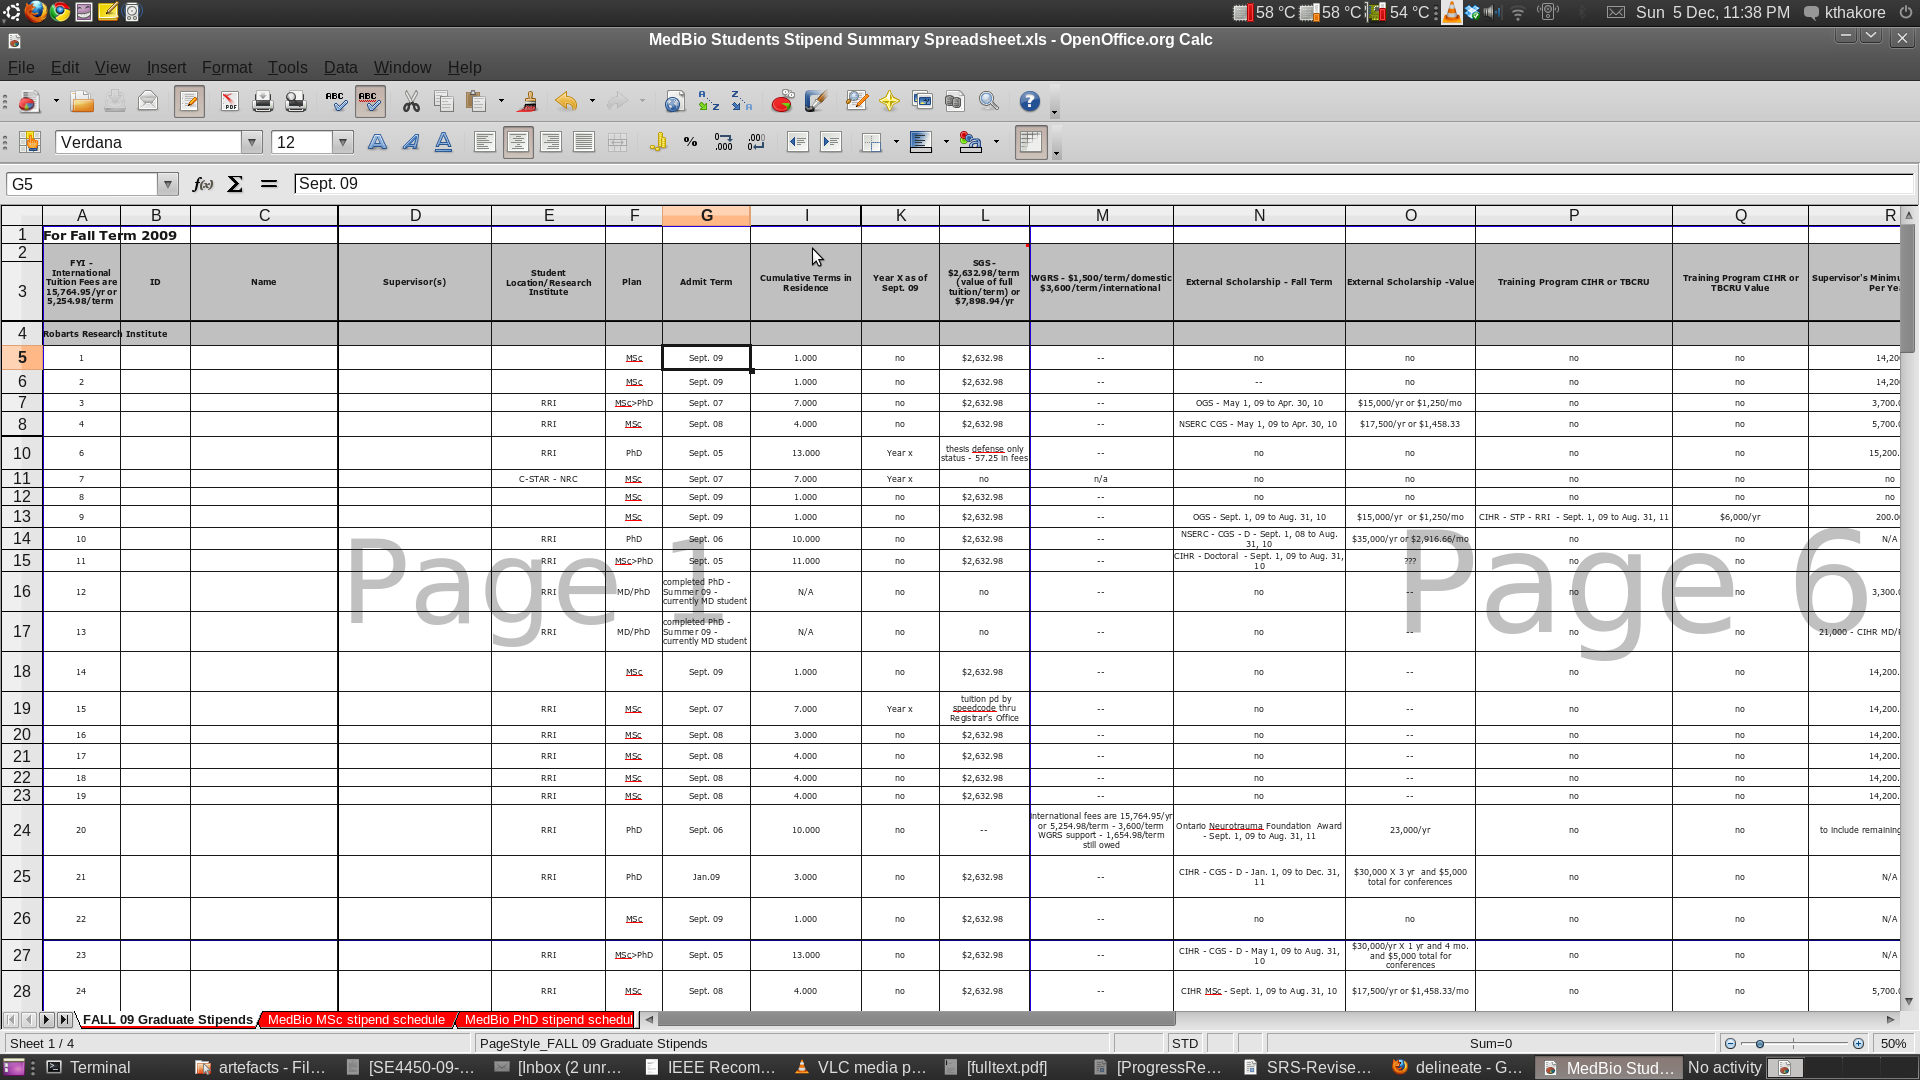
\includegraphics[scale=0.25]{diagrams/Current_System.png}
\caption{Current System}
\label{fig:Curr_Sys}
\end{figure}

\begin{figure}[htp]
\centering
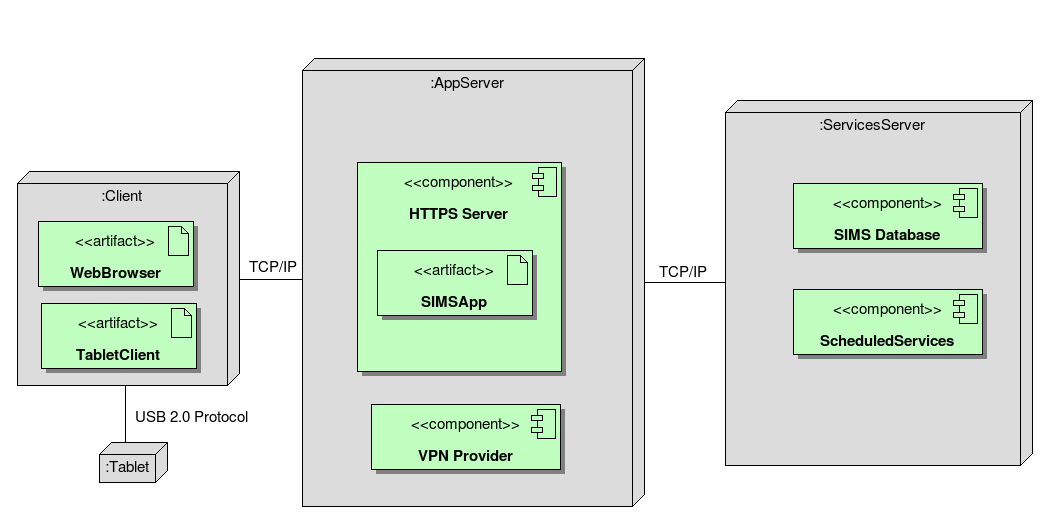
\includegraphics[scale=0.40]{diagrams/SystemOverview.png}
\caption{Proposed System}
\label{fig:New_Sys}
\end{figure}

\section{Software Requirements Specification}

\subsection{Product perspective}
The product will be self contained as it is responsible for the User Interface, Application and Data Storage.
Figure \ref{fig:New_Sys} again describes the perspective of the system.
The product will have the following constraints:
\begin{itemize}
\item User Interface: The specifications of each view of the user interface will be provided for this project.
\item Hardware Interface: The system will be using a Wacom tablet as a hardware to acquire signatures.
\item Software interfaces: The system will have to employ several software interfaces.
\begin{itemize}
\item Application Server: Apache 2.0 will be used to deploy the system with SSL security.
\item VPN Provider: OpenVPN will be used to deploy the system as a self contained virtual private
network.
\item Database Software: A PostgreSQL RDBMS server will be used to run the Data Storage Component of the Software.
\end{itemize}
\end{itemize}
\subsection{Product Function}
\subsection{User Characteristics}
Figure \ref{fig:users} describes the relation between the users of the systems, for further clarification:
\begin{itemize}
\item General User: Any user of the system, can login into the system 
\begin{itemize}
\item Faculty: Members of the faculty that can see data of several students who are not student themselves
\begin{itemize}
\item Graduate Administrator: Essentially the super user of the system, can access and modify all data 
\item Advisory Committee Member: Can view attached student data and advisory meeting documents
\item Graduate Faculty Executives: Can view all student data and view publish reports 	
\end{itemize}
\item Technical Administrator: A user that cannot access any data but can manage users 
\item Graduate Student: A student that can only view their own information and update it
\end{itemize}
\end{itemize}

\begin{figure}[htp]
\centering
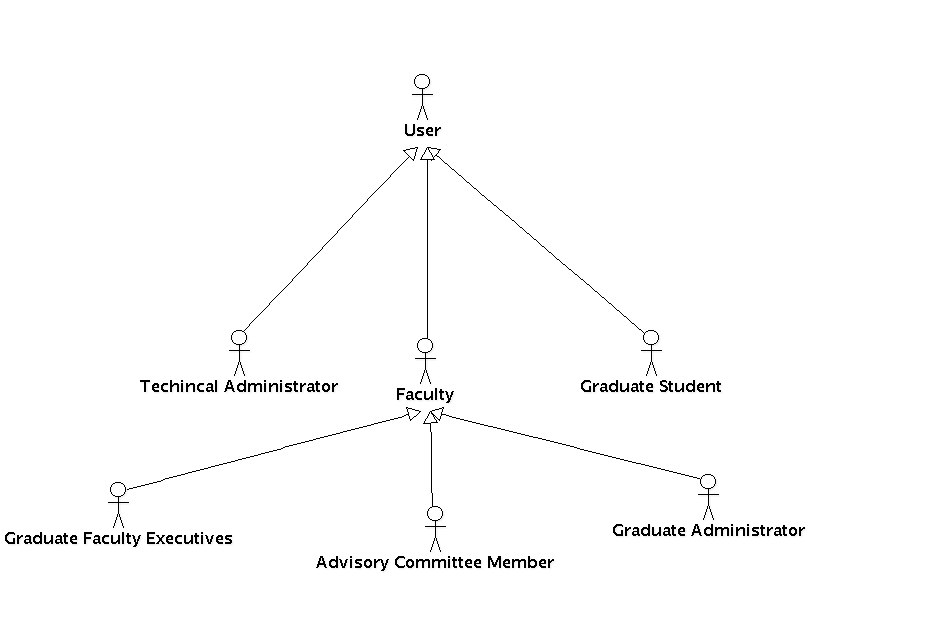
\includegraphics[scale=0.40]{diagrams/use_cases/UserHeirachy_uc.png}
\caption{Users of the System}
\label{fig:users}
\end{figure}

\subsection{Constraints}

\subsubsection{Technical Environment}
SIMS will be built on the Linux Server platform for the Database and Application Server. The client will be limited to a Linux Operating System with the Firefox 3.6 web browser.  
\subsubsection{Security}
UWO has strict guidelines (FIPPA) to handling signatures and student data. For this purpose proven technologies will be used, such as HTTP secure and VPN.
\subsubsection{Reliability of Data}
Data in SIMS is critical and needs to be protected from data losses. A regular backup of the database will help to accomplish this. 

\subsection{Assumptions and dependencies}
\subsubsection{Student Data v.s User Data}
Student Data is separate from the system, and will not be removed from the system after they graduate. However a user can still be expired from the system. Since archival is needed for a period of atleast 7 years SIMS will need to separate user access and student data. 
\subsubsection{Intrinsic Student Data}
Another assumption required by SIMS's requirement is that Student can only be stored in the system if they have a funded term attached to them. This implies that funding is tied on a term basis, which can help to simply futher calculations. 

\section{Specific Requirements}
\subsection{External interface requirements}
\subsubsection{Graphical User Interface}
A set of graphical user interfaces defined in HTML will be provided for the system to template. SIMS will show the interfaces as is and add dynamic data to them. 
\subsubsection{Hardware Interface}
SIMS will acquire signatures from client side wacom tablets from a USB 2.0 protocol. Data will be outputted in a BMP file format. 

\begin{figure}[htp]
\centering
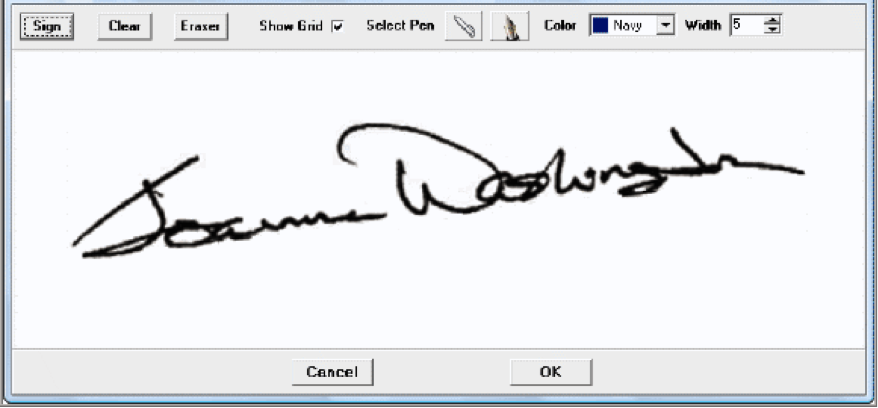
\includegraphics[scale=0.75]{diagrams/HTMLTemplating/Figure6.png}
\caption{Signature Interface View}
\label{fig:signature}
\end{figure}

\begin{itemize}
\item Purpose: To provide an interface for recording advisory committee member signatures.
\item Response Sequence: When the e-signature pad is connected to the device, it will automatically start the e-signature interface which records an individual signature.
\item Associated Functional Requirements:
\begin{itemize}
\item Clear: Ability to clear the signature if the signer does not accept the signature
\item Sign: Once the output on the screen is satisfactory, the user can "Sign" the document which will save the image into the document and link it to the current document.
\end{itemize}
\end{itemize}
\subsection{Functional requirements}
\subsubsection{User Administration}

\begin{figure}[htp]
\centering
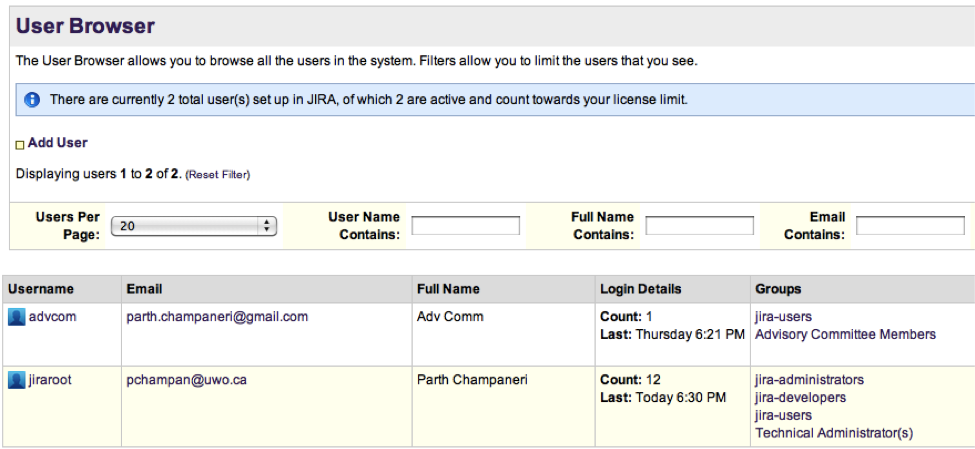
\includegraphics[scale=1]{diagrams/HTMLTemplating/Figure7.png}
\caption{User Browser}
\label{fig:UserBrowser}
\end{figure}


\begin{itemize}
\item Purpose: The user browser lists all the users in the system for technical administration. 
\item Response Sequence: Login and click on User Browser from the administration Dashboard. From this page, the administrator can perform the following functions:
\item Associated Functional Requirements:
\begin{itemize}
\item Create new users: Adding a new user to the system can only be accomplished by the Technical Administrator after an approval from the Graduate Administrator. 
\begin{figure}[htp]
\centering
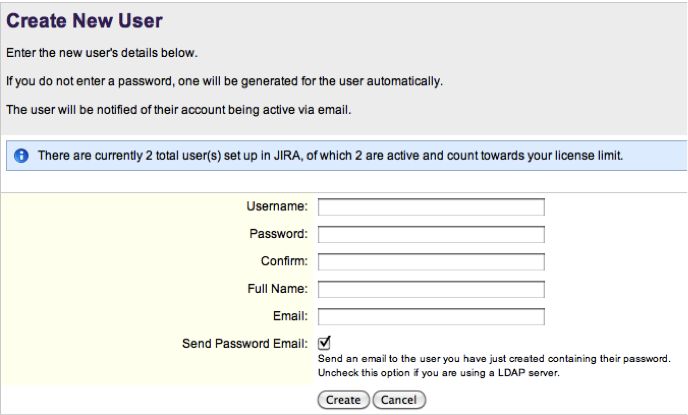
\includegraphics[scale=1]{diagrams/HTMLTemplating/Figure8.png}
\caption{New Users}
\label{fig:NewUser}
\end{figure}
\item Adding new user roles: User roles are primary stakeholder groups for the system. Currently, our primary stakeholders are Advisory Committee Members, Graduate Administrators, Graduate Executives, and Graduate Students.
\begin{figure}[htp]
\centering
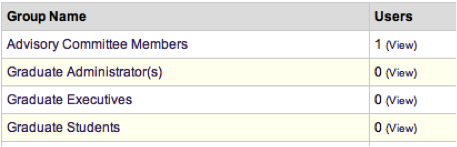
\includegraphics[scale=1]{diagrams/HTMLTemplating/Figure9.png}
\caption{New Users Roles}
\label{fig:NewUserRoles}
\end{figure}

\item Adding Operation to roles: Permissions can be added to the user permission list by clicking on the Add New permission button under User Administration. This can be done by the Technical Administrator.

\begin{figure}[htp]
\centering
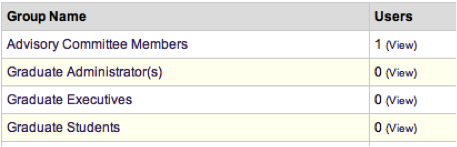
\includegraphics[scale=1]{diagrams/HTMLTemplating/Figure9.png}
\caption{New Operations}
\label{fig:NewPermission}
\end{figure}


\end{itemize}
\end{itemize}

\subsubsection{System Wide Login Page}

\begin{figure}[htp]
\centering
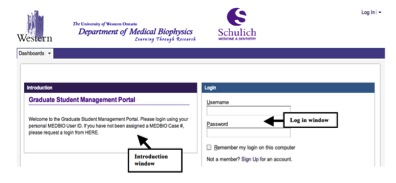
\includegraphics[scale=1]{diagrams/HTMLTemplating/Figure1.jpg}
\caption{System Wide Login Page}
\label{fig:SystemWideLogin}
\end{figure}


\begin{itemize}
\item Purpose: Provide a universal log-in page to provide access to the end users of the system
\item Response Sequence: In order to access the login page, user will have to type the system URL in a supported browser, which will direct them to this log in page. 
\item Associated Functional Requirements: 
\begin {itemize} 
\item Introduction widget: This widget will provide a short introduction to the purpose of the management system. It will also feature an Important Links section with a link to the website of The Department of Medical Biophysics. Furthermore, a link to a technical troubleshooting page will be created.
\item Login window: This is the actual login page where the user will enter their credentials to login. Users cannot sign up for the system individually. The Graduate Administrator facilitates the sign up process and a direct link to request the login credentials will be set up.
\end{itemize}
\end{itemize}


\subsubsection{System Dashboard}
\begin{figure}[htp]
\centering
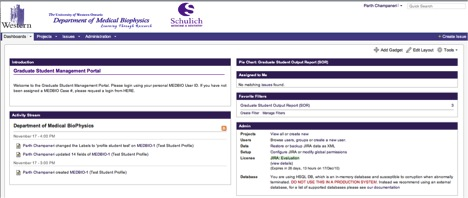
\includegraphics[scale=1]{diagrams/HTMLTemplating/Figure2.jpg}
\caption{System Dashboard Page}
\label{fig:SystemDashBoard}
\end{figure}

\begin{itemize}
\item Purpose: Provide a centralized location of all system functions while preserving ease of use and accessibility.
\item Response sequence: The user will be directed to this page after login.
\item Associated Functional Requirements:
\begin{itemize}
\item Provide various plugins on the Dashboard based on different user roles and operation for access to student profiles and various system features. 
\item Search: Be able to search a students profile from the Dashboard.
\end{itemize}
\end{itemize}

\subsubsection{Student Profile}
\begin{figure}[htp]
\centering
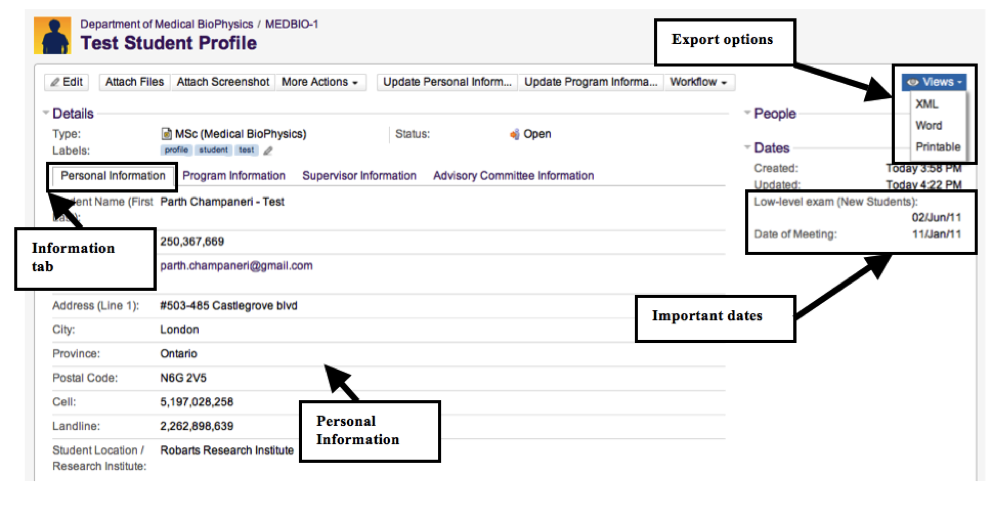
\includegraphics[scale=1]{diagrams/HTMLTemplating/Figure3.png}
\caption{Student Profile Page}
\label{fig:StudentProfile}
\end{figure}

\begin{figure}[htp]
\centering
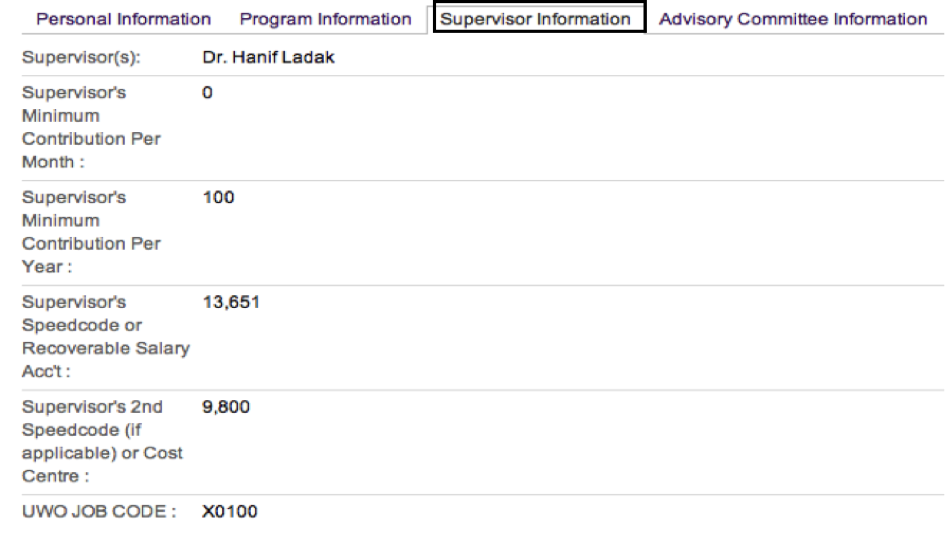
\includegraphics[scale=1]{diagrams/HTMLTemplating/Figure4.png}
\caption{Supervisor Information Page}
\label{fig:SuperInfo}
\end{figure}


\begin{itemize}
\item Purpose: Provide an intuitive dossier format interface for users to see the student profile in a centralized location. The key goal is to ensure that all the important system functionality is in a centralized location. Note the attached sample HTML page.
\item Response sequence: In order to access the GUI, the user will be required to login and will be taken to a Dashboard which will have options to generate reports and search a student by their assigned id. Once selected the user will be able to see a student profile and be able to perform various functions based on their authentication scope as defined in the access control list.
\item Associated Functional Requirements:
\begin{itemize}
\item Information Tab Section: The profile page will feature information tabs with centralized information about their Personal Information, Program Information, Supervisor Information and Advisory Committee Meeting Information. 
\item Supervisor Information: This tab contains information regarding a students' direct Supervisor Name and information about the supervisors minimum student contribution along with other logistical information. This information is created with the sample Medical Biophysics excel sheet provided by the Graduate Administrator user at the Department of Medical Biophysics.	

\item Expansion: Each section can be clicked on to show summary of additional information
\item Link:  Each information tab will link to another section pages (if applicable)
\item Grouping: Group Dates and people in the same window area for better accessibility
Export Options: There should be an export option to ensure that a user can export their entire student profile in Word, PDF and a printable HTML.
\item Attachment Options: The dossier should feature an attachment tab that includes all relevant attachments/forms for that student profile.
\end{itemize}
\end{itemize}

\subsubsection{Graduate Student's Personal Information}
\begin{itemize}
\item Graduate Student's Personal Information:
Contains data regarding the students contact information including their UWO e-mail address and their current location. This system feature is to document how personal information is stored and accessed via different user roles. 
\item Graduate Students: Graduate Students can view their entire profile which includes information on their program, supervisor, advisory committee, as well as any personal records. Data access is restricted only to their personal profile.
\item Graduate Administrator: Ability to edit all fields.
\item Graduate Executives and Advisory Committee members: Read only access.
\item Update Personal information
\begin{itemize}
\item Visibility: Graduate students only
\item Restrictions: Only allowed to update contact information and address. 
\item Usability: Graduate administrator is responsible for inputting student data.
\end{itemize}
\end{itemize}
\subsubsection{Graduate Students’ Program Information}

\begin{figure}[htp]
\centering
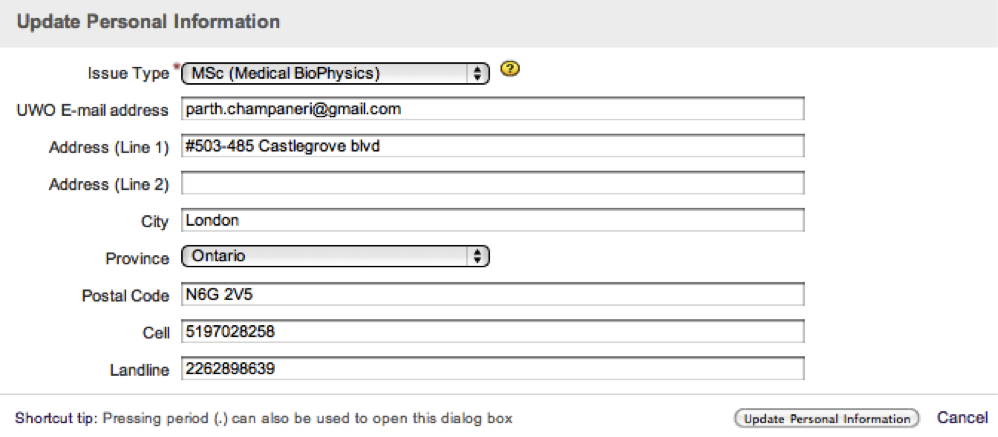
\includegraphics[scale=1]{diagrams/HTMLTemplating/UpdatePersonalInfoStudent.png}
\caption{Update Personal Information Student}
\label{fig:UpdatePIS}
\end{figure}

\begin{itemize}

\item Contains information related directly to the students program enrollment. Information includes Admission Term and Year, Thesis information, Publications (if any) and a custom field that records if the student has indicated MSc to PhD reclassification.
\item Update Program Information
\begin{itemize}
\item Visibility: Graduate students only
\item Restrictions: Allowed to update Publications, Thesis (if applicable) and Low-Level exam date if known. 
\end {itemize} 
\end {itemize} 

\subsubsection{Graduate Students' Advisory Committee}
\begin{itemize}
\item Advisory Committee Information tab is a centralized location for all advisory committee information which has taken place for a student. Under this tab, pertaining information such as the list of all advisory meetings, evaluation of a particular advisory meeting whether it was satisfactory or unsatisfactory and any supervisor/member recommendations after the meeting. Advisory committee is a progression requirement which happens for each student atleast once a year. Scheduling is usually done by the student or by the graduate administrator. One of the key requirements is to track and remind students of their advisory meeting output and ensure that a post-meeting report is generated to satisfy their progression requirements.

\begin{figure}[htp]
\centering
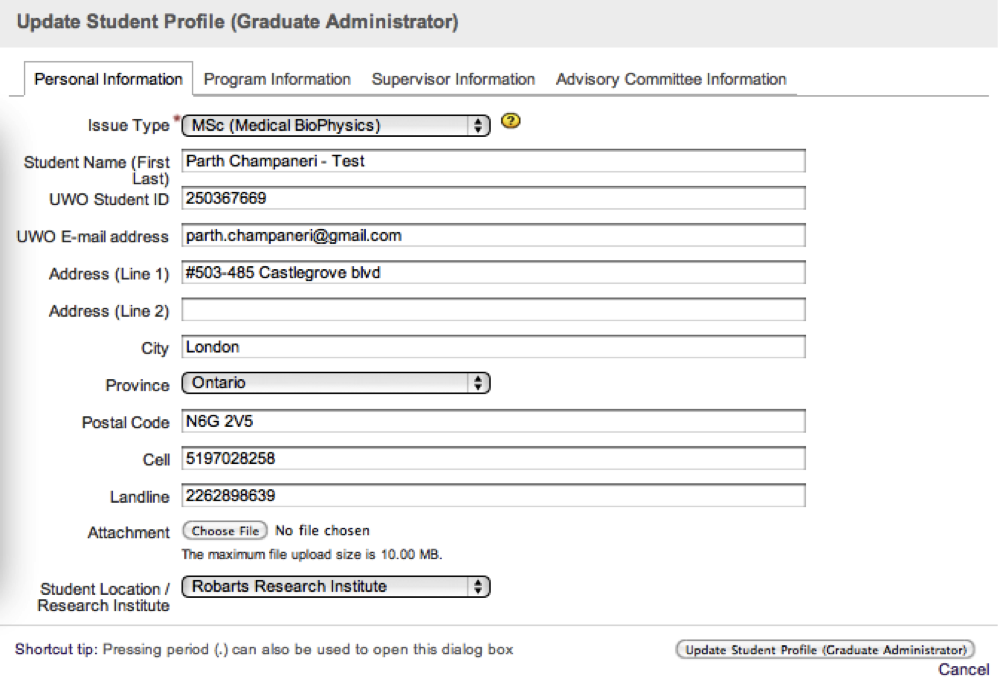
\includegraphics[scale=1]{diagrams/HTMLTemplating/UpdateStudentProfileAdmin.png}
\caption{Update Advisory Committee Information}
\label{fig:UpdateACI}
\end{figure}

\item Update Advisory Committee Information
\begin{itemize}
\item Visibility: Graduate students and Graduate Administrator
\item Restrictions: Allowed to update names of supervisor and advisors after a date for the meeting has been formed.
\end{itemize}
\item Comment on Advisory Committee Meeting:

\begin{figure}[htp]
\centering
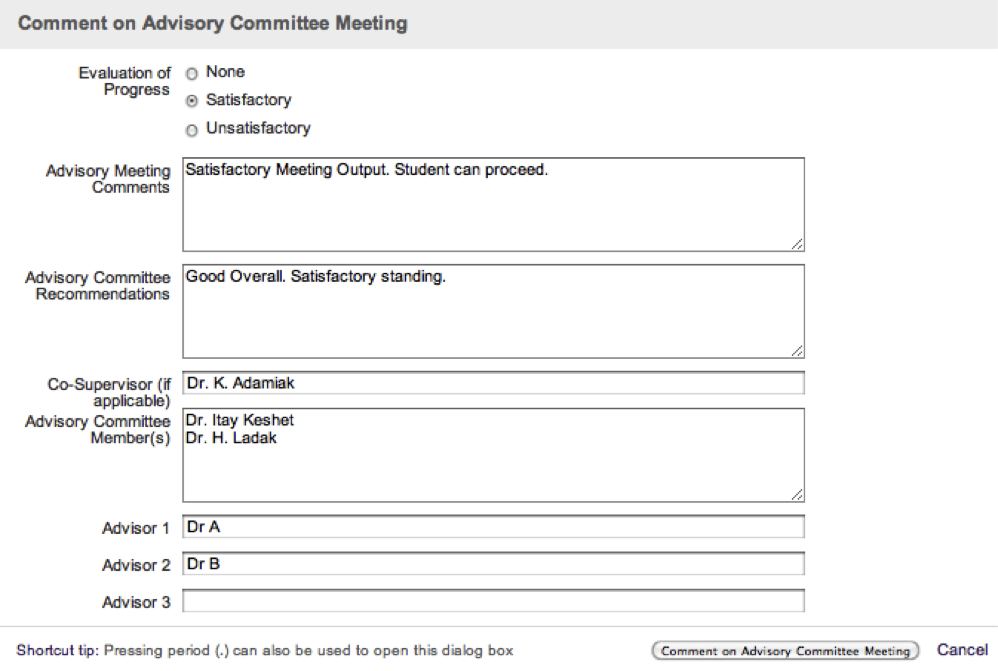
\includegraphics[scale=1]{diagrams/HTMLTemplating/CommentAdvisory.png}
\caption{Adding Comments to Advisory meetings}
\label{fig:UpdateCAM}
\end{figure}

\begin{itemize}
\item Visibility: Advisory Committee Members
\item Restrictions: Cannot access any other data. Members can update progress and output of the meeting. Can also provide recommendations and comments.
\end{itemize}
\end{itemize}

\subsubsection{Data Reporting}
\begin{itemize}
\item Queries: Reports can be generated by filtering via various fields or by entering customized queries in the reporting interface.
\item Queries can be run by the administrator, advisory members and graduate executives.
\item Sample Student Profile Report (Word): Users can export student profile in a Word document which contains all the information regarding the selected student. The scope of the document generated will be restricted to the roles and permission of the user.
\item Sample Graduate Student Output Report (SOR) - Excel: Users can export a SOR based on custom queries which are either preset or custom created.

\begin{figure}[htp]
\centering
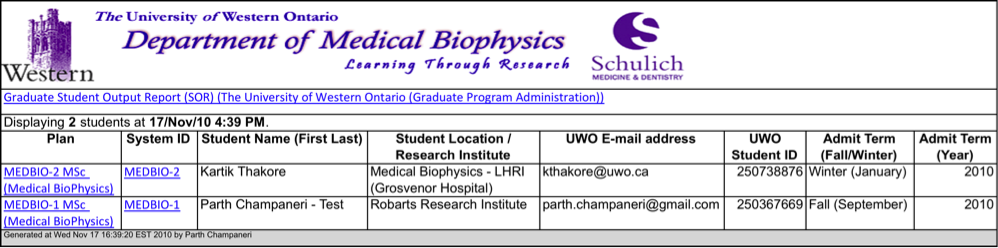
\includegraphics[scale=1]{diagrams/HTMLTemplating/SOR_Excel.png}
\caption{Excel Graduate SOR Report}
\label{fig:ExcelSOR}
\end{figure}

\item Custom Pie Charts: Pie charts and trend charts can be generated based on the SOR or a custom query.

\begin{figure}[htp]
\centering
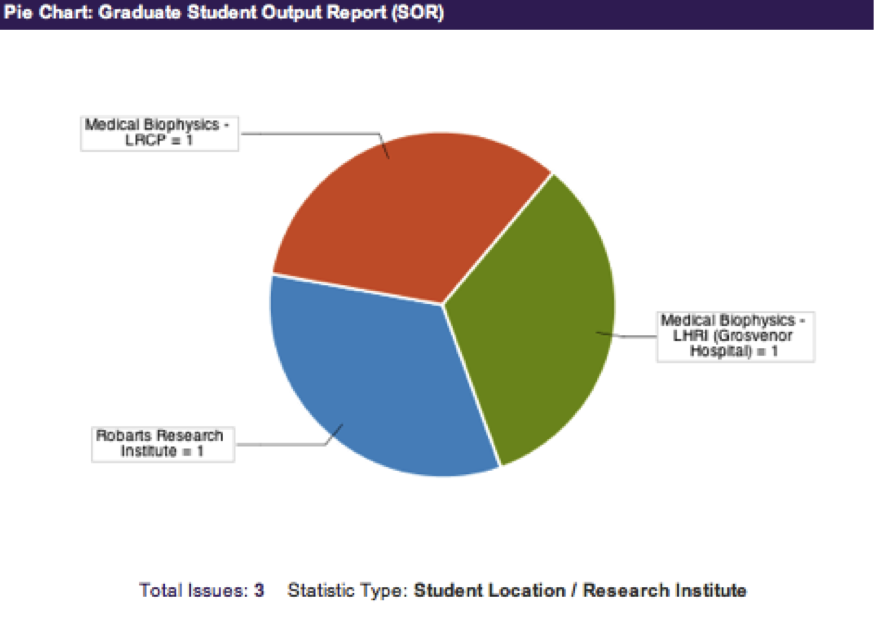
\includegraphics[scale=1]{diagrams/HTMLTemplating/PieChart.png}
\caption{Excel Graduate SOR Pie Chart}
\label{fig:PieSOR}
\end{figure}

:\end{itemize}

\chapter{Design}
\section{Iteration 1}

The first iteration focused on completing the analysis of the user use cases, understanding the data flow of the system. Finally based on the analysis a MVC architecture was designed and implementation. The implementation focused on :

\begin{itemize}
\item Student Data Representation 
\item Framework to display HTML templates
\item Authentication Data Representation 
\end{itemize}

\section{Analysis}

\subsection{User Hierarchy}
As specified in the SRS the user hierarchy is well defined in Figure \ref{fig:users}. Looking at the user interface provided the following use cases can be 
defined.

\subsection{Use Cases}

\subsubsection{Generic User}

\begin{figure}[htp]
\centering
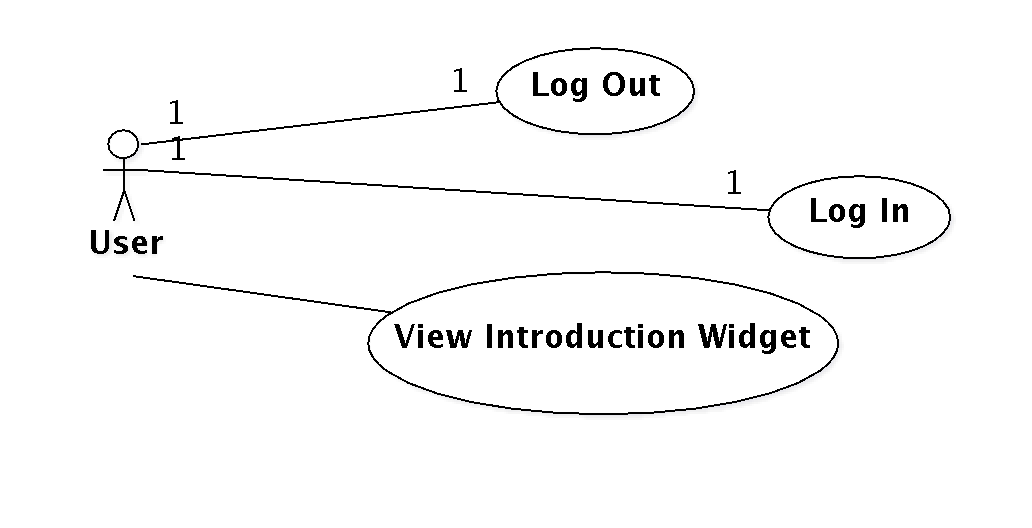
\includegraphics[scale=0.25]{diagrams/use_cases/User_uc.png}
\caption{Generic User Use Case}
\label{fig:UserLog}
\end{figure}

Figure \ref{fig:UserLog} defines the use cases of any user of the system. The user will be able to login and logut.

\subsubsection{Dashboard}

\begin{figure}[htp]
\centering
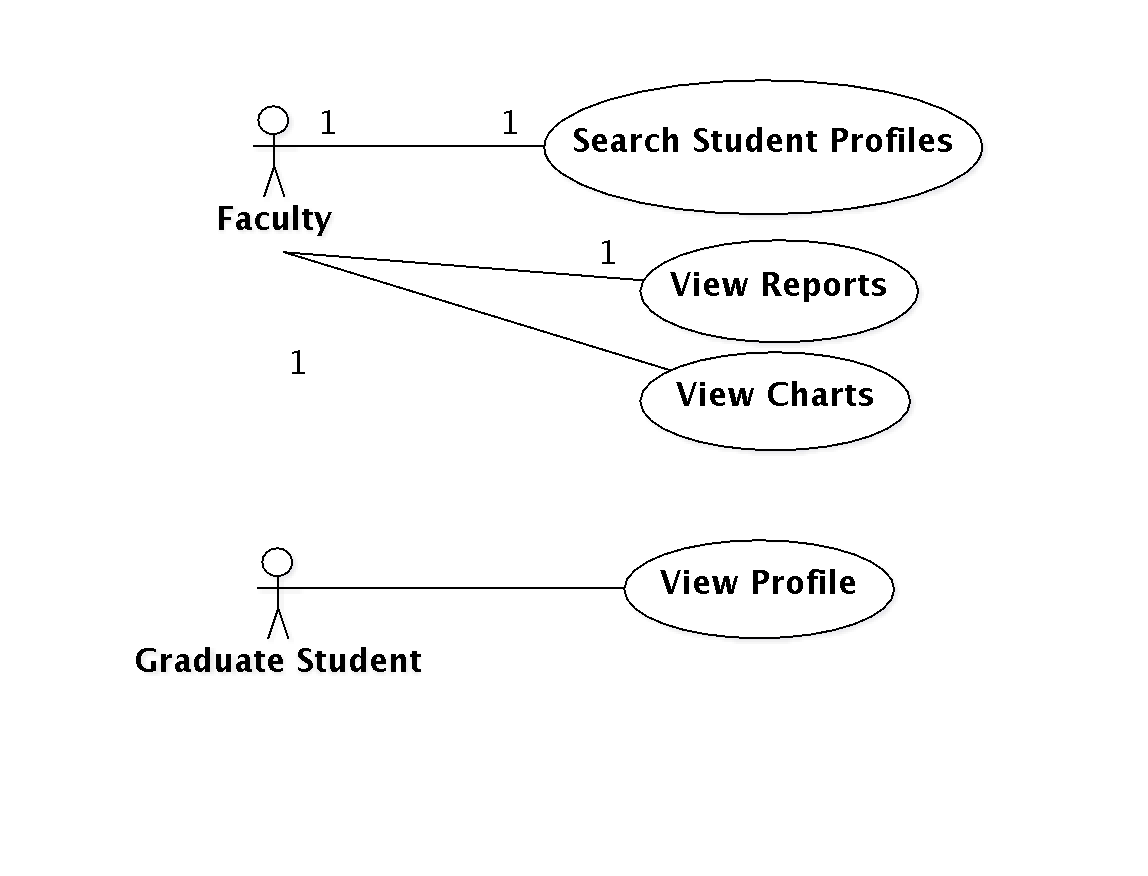
\includegraphics[scale=0.25]{diagrams/use_cases/Dashboard_uc.png}
\caption{Dashboard Use Case}
\label{fig:Dashboard}
\end{figure}

Figure \ref{fig:Dashboard} defines the use cases on the Dashboard features for each user.

\subsubsection{User Administration}

\begin{figure}[htp]
\centering
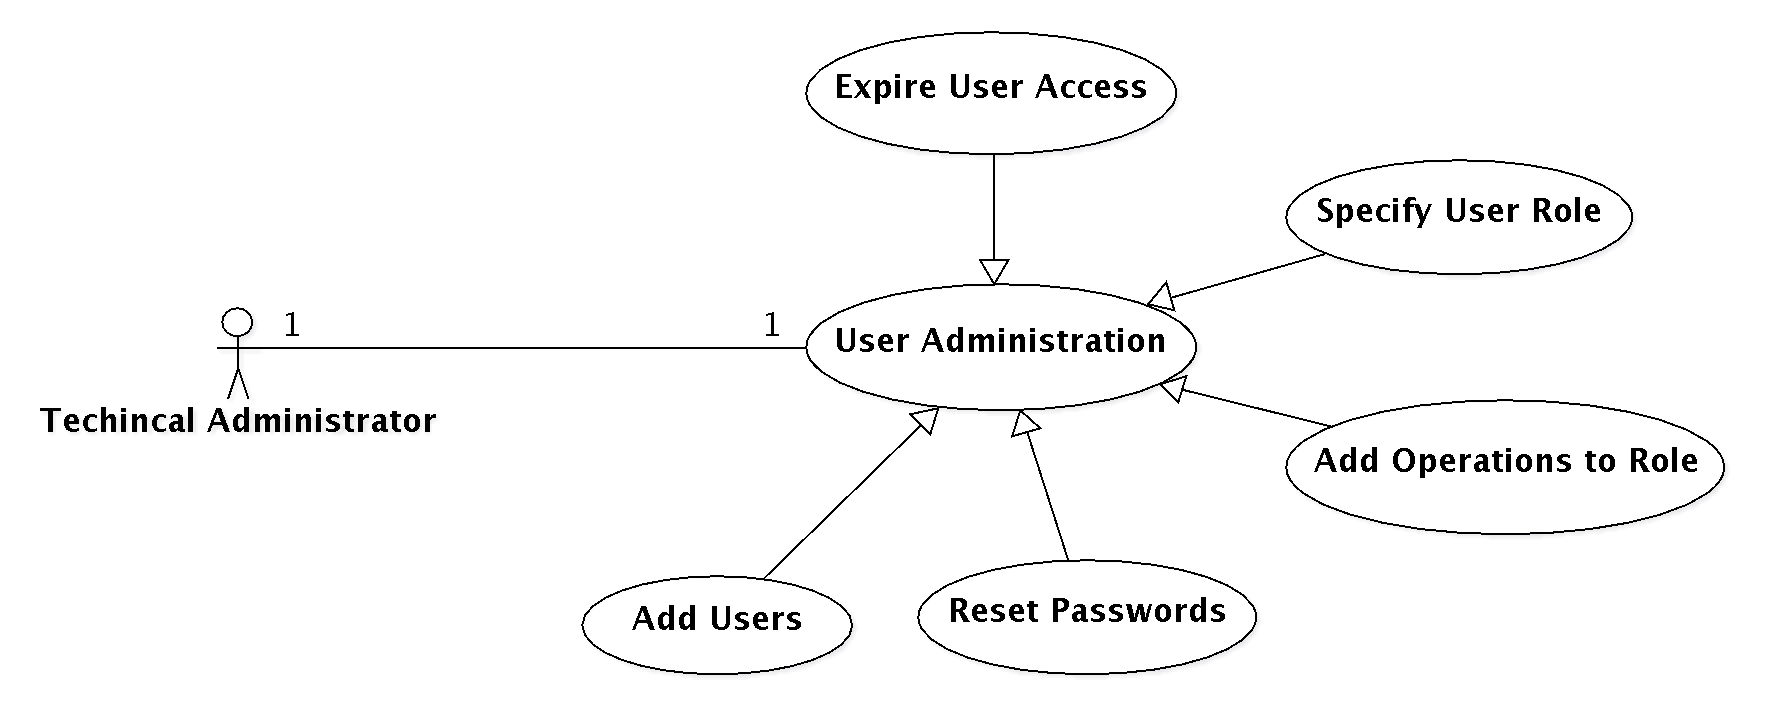
\includegraphics[scale=0.25]{diagrams/use_cases/TechAdmin_uc.png}
\caption{User Administration Use Case}
\label{fig:UserAdmin}
\end{figure}

Figure \ref{fig:UserAdmin} defines the use cases to do user administrator. 

\subsubsection{Student Data Access}
\begin{figure}[htp]
\centering
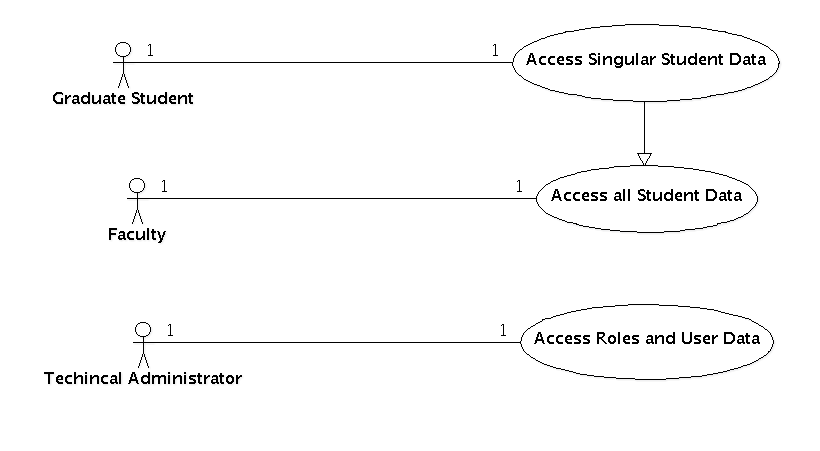
\includegraphics[scale=0.5]{diagrams/use_cases/access_uc.png}
\caption{Data Access Use Case}
\label{fig:UserAccess}
\end{figure}

Figure \ref{fig:UserAccess} defines the use cases that determines the access level on the student data.

\begin{figure}[htp]
\centering
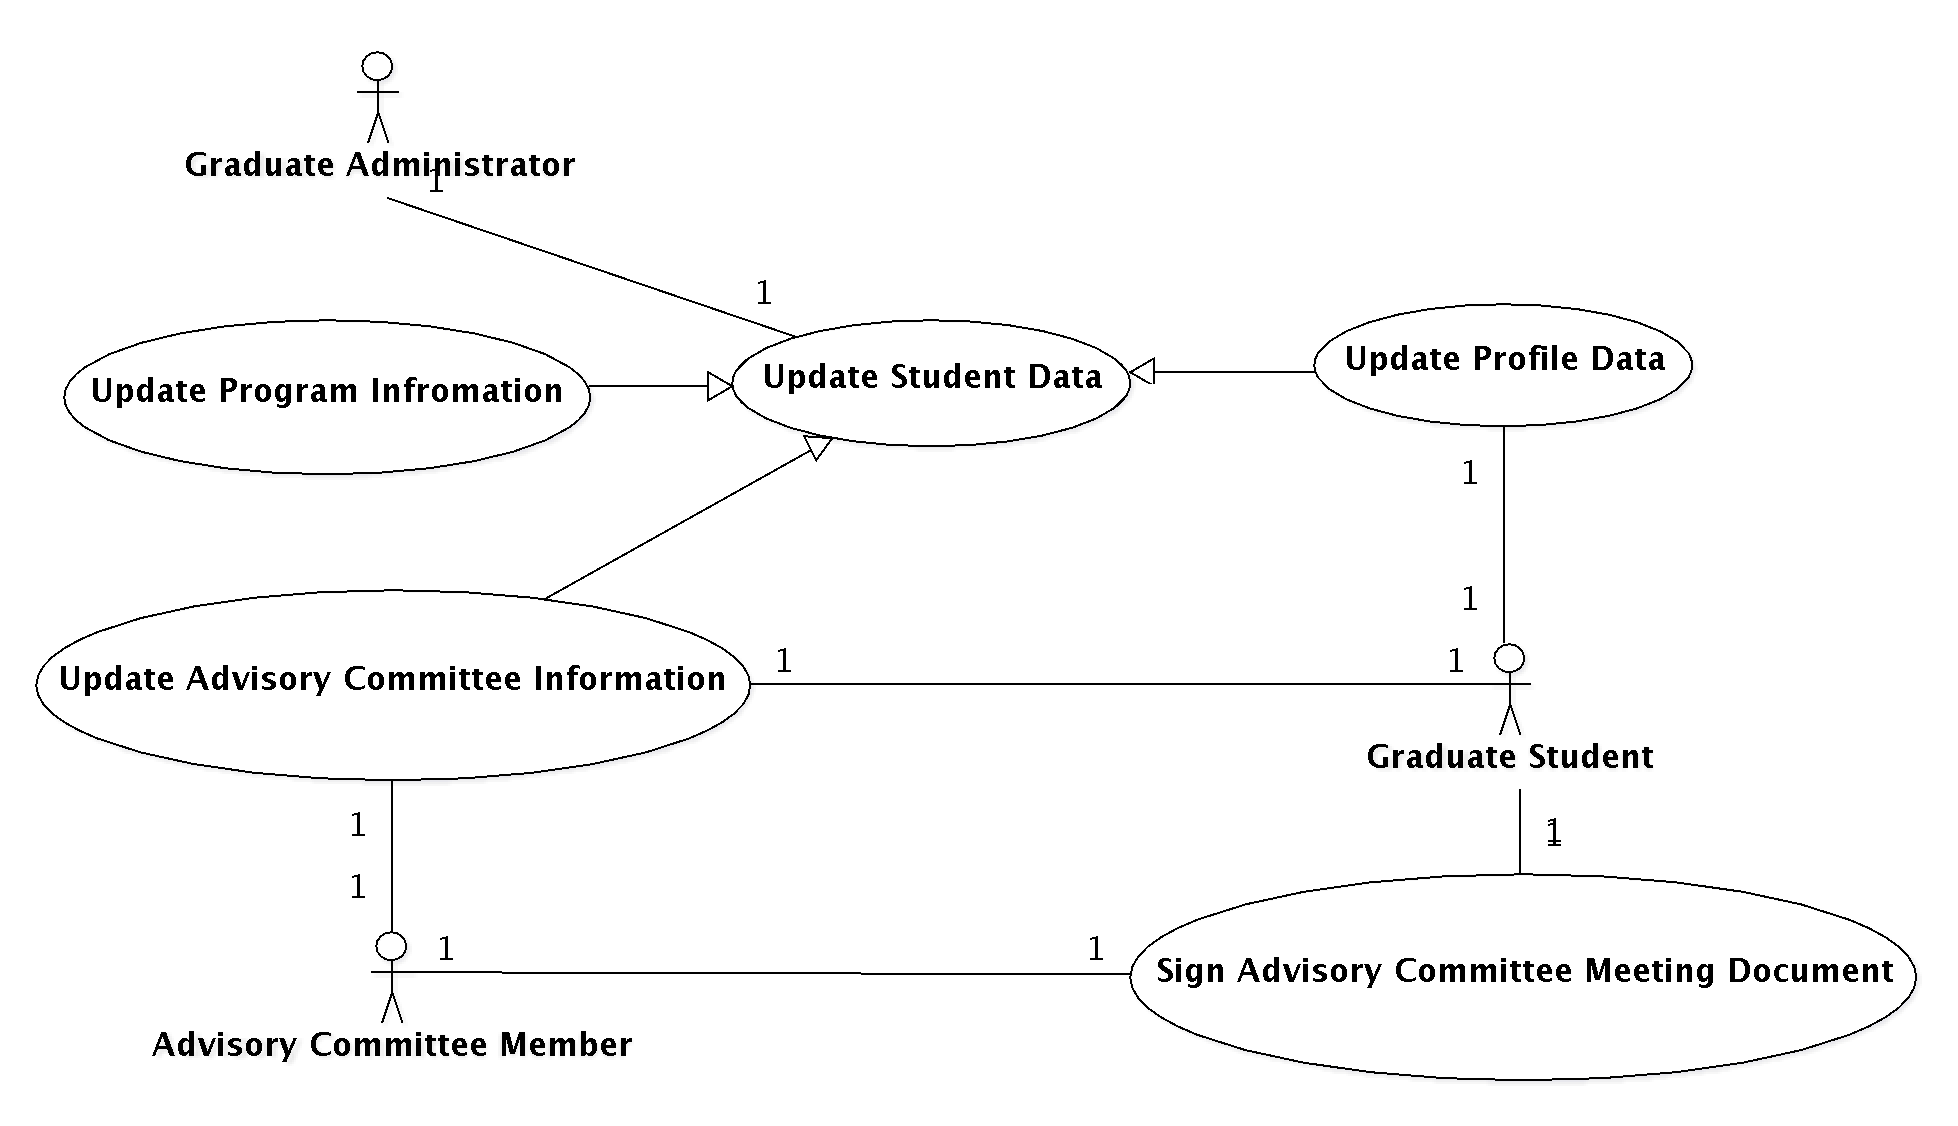
\includegraphics[scale=0.25]{diagrams/use_cases/system_data_uc.png}
\caption{System Data Use Case}
\label{fig:SystemData}
\end{figure}

Figure \ref{fig:SystemData} defines modifications that can be done by the Graduate Administrator. 

\subsubsection{Triggers and Reporting}
\begin{figure}[htp]
\centering
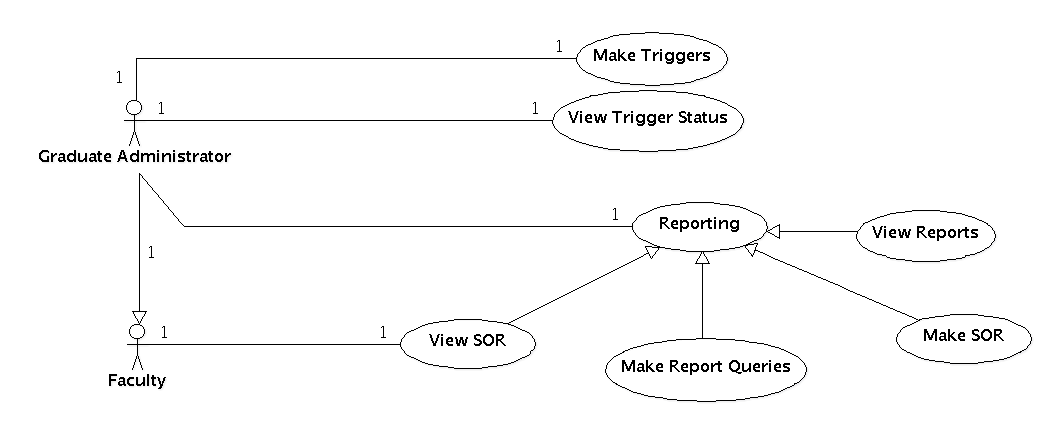
\includegraphics[scale=0.5]{diagrams/use_cases/triggers_uc.png}
\caption{Triggers and Reporting Use Case}
\label{fig:Triggers}
\end{figure}

Figure \ref{fig:Triggers} describe the functionality access for providing triggers and reporting. 

\subsection{ Data Flow Considerations }

\begin{figure}[htp]
\centering
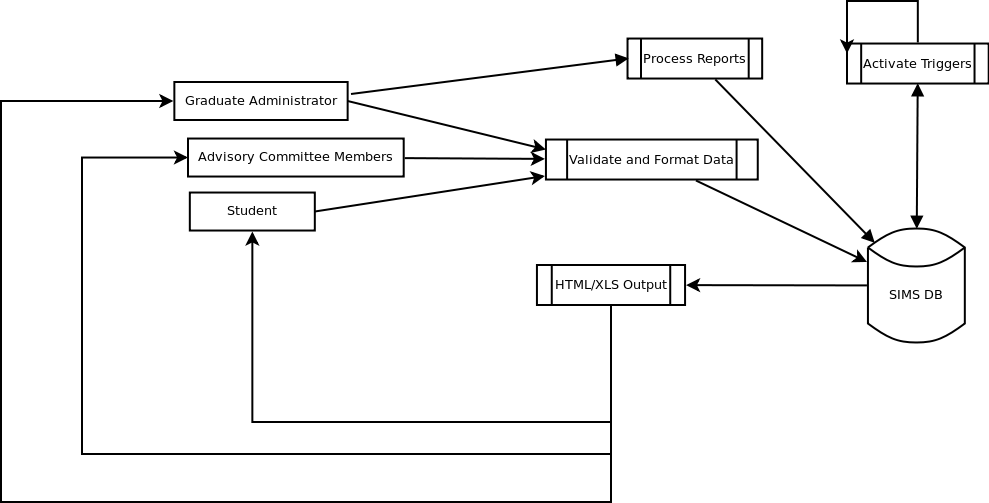
\includegraphics[scale=0.5]{diagrams/data_flow/dataflowdiagram.png}
\caption{Data Flow of the System}
\label{fig:DataFlow}
\end{figure}

Figure \ref{fig:DataFlow} describes the data flow analysis of the system. 

\begin{figure}[htp]                                                             
\centering                                                                      
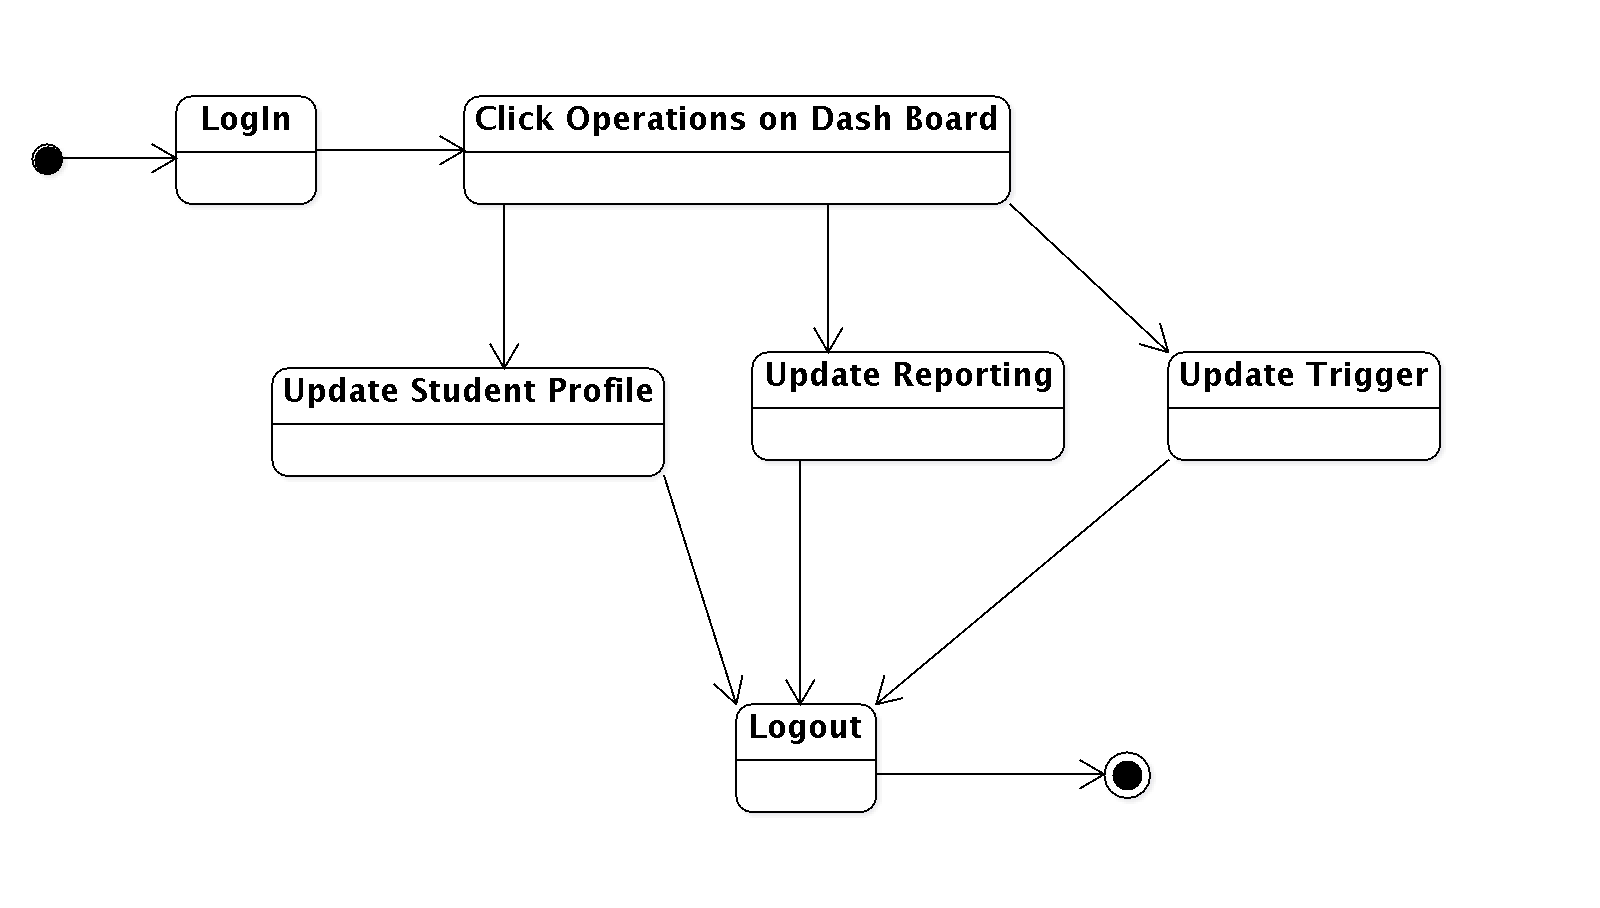
\includegraphics[scale=0.25]{diagrams/statechart_uc.png}
\caption{Transitions through the System Interface}                              
\label{fig:Transitions}   
\end{figure}                                                                    
             
Figure \ref{fig:Transitions} describe the generic user transitions through the systems. 


\section{Software Design Specification}

\subsection{Server Analysis and Design}
One of the critical requirements of the system is to meet FIPPA standards. 
\subsubsection{SSL HTTP Server}

The server architecture would require a HTTP/SSL server to provide the standard security protocol with a signed Thawte SSL certificate expected from UWO ITS standards \cite{ITS}.

\subsubsection{Application Server}

The application server would run as a separate user ( Unix User ) then the HTTP/SSL Server. Additionally to provide access to the application, it will be proxied to the HTTP/SSL Server. 
Finally the Application Server directly would need to communicate with a Database Server and the Cache Server, therefore it will be place on the same machine.

\subsubsection{Database Server}

According to FIPPA:
\begin{quote}
Public bodies have certain obligations and duties under FIPPA.  Broadly speaking, these duties relate to responding to access requests, protecting personal information ... \cite{FIPPA}
\end{quote}
Therefore the Database Server selected must be able to handle requests reasonably and scaled well for future needs. Additionally for security considerations the Database Server would just be able to 
communicate locally with the application server. Lastly a Relational Database is required so as to meet the considerations of the business rules employed in Graduate Programs. 

\subsubsection{Cache Server}

The Cache server is responsible of holding user session data securely and separately from the Database server. This meets the requirements of FIPPA mentioned above because user session data is volatile and doesn't scale well in a Relational Database. The extra load from user sessions could lead to Denial of Service attacks, which would be in violation of FIPPA. 

\subsection{Application Framework}

To meet the requirements of being flexible and powerful enough to handle various business requirements, a REST application framework is selected. A REST application provides a consistent server state by providing chained actions. A user can traverse through links to perform several actions. This model works well with the requirements of a student tracking software, as the graduate assistant performs actions on student profiles, meetings, reports etc. REST is based on the messaging design pattern which allows the design of each URL to act as clear messages indicating the server state. This design makes testing easier and debugging simpler. In addition it forces code to be decoupled, reusable and encapsulated from the start \cite{REST}. Applying this system in the real world would thus ensure some code quality. Finally the REST framework also separates 

\subsubsection{User Session}

Based on the User Hierarchy and it Use Cases there is a direct need for the application to handle user authentication and authorization per response done. This is handled simply by a REST message design pattern. Before each response is handled it is 'chained' to a root method that checks for the user session data and confirms authorization and authentication.  

\subsubsection{Data Abstraction Schema}

The framework should also abstract the database tables due to reporting requirements and being able to apply new business rules quickly. By abstracting the database tables into a high level code and interface, very simple code can be written to CRUD ( CREATE, READ, UPDATE, DELETE ) any data in the system. 

\subsubsection{Report Generation}
Finally for the preliminary requirements of report generation a PDF generator plug-in is required from the framework. More format should be available and easily implementable. 

\subsection{User Interface}
Since most of the system will be accessed through the web browser a feasible technology that can be used is Javascript/HTML.  

\subsection{Class Design}

Classes are seperated in 3 categories: Model, View, and Controller. Classes can be initiated as runtime instances as needed by a request. 

\begin{tabular}{| l | p{7cm} |}
\hline
 Class                                                           & Purpose and URL \\
\hline
\hline
 SIMS::Controller::AdvCommMember                                 &  Handles specific urls (actions) for advisory committee members. (\verb+\advcommember+) \\ \hline
 SIMS::Controller::Faculty                                       &  Handles specific urls for all faculty members. (\verb+\faculty+) \\ \hline
 SIMS::Controller::GraduateAdmin                                 &  Handles specific urls for the graduate admin (\verb+\gradadmin+) \\ \hline
 SIMS::Controller::GraduateExec                                  &  Handles specific urls for the graduate executive user (\verb+\gradeexec+) \\ \hline
 SIMS::Controller::Helper                                        &  A helper class for sending email confirmation and other static methods \\ \hline
 SIMS::Controller::Login                                         &  Handles the login form (\verb+\login+) \\ \hline
 SIMS::Controller::Logout                                        &  Handles user session destruction (\verb+\logout+) \\ \hline
 SIMS::Controller::Meeting                                       &  Handles meeting urls for authorized users (\verb+\meeting+) \\ \hline
 SIMS::Controller::Report                                        &  Handles report generation for grad admin (\verb+\report+) \\ \hline
 SIMS::Controller::Root                                          &  The base class that checks for user sessions on and provides the user dashboard feature (\verb+\+) \\ \hline
 SIMS::Controller::Student                                       &  Handles specific urls for the student user (\verb+\student+) \\ \hline
 SIMS::Controller::TechAdmin                                     &  Handles sepcific urls for the technical admin user (\verb+\techadmin+) \\ \hline
 SIMS::Model::DB                                                 &  Connects to the database server \\ \hline
 SIMS::Model::DB::Event                                          &  Model abstraction for respective table\\ \hline
 SIMS::Model::DB::Fund                                           & Model abstraction for respective table\\ \hline
 SIMS::Model::DB::Meeting                                        & Model abstraction for respective table\\ \hline
 SIMS::Model::DB::MeetingAdvisor                                 & Model abstraction for respective table\\ \hline
 SIMS::Model::DB::MeetingComment                                 & Model abstraction for respective table\\ \hline
 SIMS::Model::DB::MeetingConfirmation                            & Model abstraction for respective table\\ \hline
 SIMS::Model::DB::Plan                                           & Model abstraction for respective table\\ \hline
 SIMS::Model::DB::PlanStudent                                    & Model abstraction for respective table\\ \hline
 SIMS::Model::DB::Report                                         & Model abstraction for respective table\\ \hline
 SIMS::Model::DB::Role                                           & Model abstraction for respective table\\ \hline
 SIMS::Model::DB::Student                                        & Model abstraction for respective table\\ \hline
 SIMS::Model::DB::StudentSupervisor                              & Model abstraction for respective table\\ \hline
 SIMS::Model::DB::Supervisor                                     & Model abstraction for respective table\\ \hline
 SIMS::Model::DB::Term                                           & Model abstraction for respective table\\ \hline
 SIMS::Model::DB::TermFunding                                    & Model abstraction for respective table\\ \hline
 SIMS::Model::DB::TermStudent                                    & Model abstraction for respective table\\ \hline
 SIMS::Model::DB::User                                           & Model abstraction for respective table\\ \hline
 SIMS::Model::DB::UserRole                                       & Model abstraction for respective table\\ \hline
 SIMS::View::PDF::Reuse                                          & Generates PDF forms\\ \hline
 SIMS::View::TT                                                  & Convert stash data and template to HTML and JS\\ \hline
\hline
\end{tabular}

\subsubsection{Actions}
Each of the controller classes have chained actions that map to specific URL ( Path Spec ) types. 

\begin{verbatim}
.-------------------------------------+--------------------------------------.
| Path Spec                           | Action                               |
+-------------------------------------+--------------------------------------+
| /advcommmember/meeting              | /advcommmember/base (0)              |
|                                     | => /advcommmember/adv_meeting        |
| /advcommmember                      | /advcommmember/base (0)              |
|                                     | => /advcommmember/index              |
| /faculty                            | /faculty/base (0)                    |
|                                     | => /faculty/index                    |
| /faculty/search_student             | /faculty/base (0)                    |
|                                     | => /faculty/search_student           |
| /faculty/view_report                | /faculty/base (0)                    |
|                                     | => /faculty/view_report              |
| /faculty/view_student/*             | /faculty/base (0)                    |
|                                     | => /faculty/view_student             |
| /graduateadmin/add_funding/*/*      | /graduateadmin/base (0)              |
|                                     | => /graduateadmin/add_funding        |
| /graduateadmin/add_plan/*           | /graduateadmin/base (0)              |
|                                     | => /graduateadmin/add_plan           |
| /graduateadmin/add_term/*           | /graduateadmin/base (0)              |
|                                     | => /graduateadmin/add_term           |
| /graduateadmin/assign_supervisor/*- | /graduateadmin/base (0)              |
| /*                                  |                                      |
|                                     | => /graduateadmin/assign_supervisor  |
| /graduateadmin/edit_student/*       | /graduateadmin/base (0)              |
|                                     | => /graduateadmin/edit_student       |
| /graduateadmin/edit_supervisor      | /graduateadmin/base (0)              |
|                                     | => /graduateadmin/edit_supervisor    |
| /graduateadmin                      | /graduateadmin/base (0)              |
|                                     | => /graduateadmin/index              |
| /graduateadmin/supervisors          | /graduateadmin/base (0)              |
|                                     | => /graduateadmin/supervisors        |
| /meeting/*/add_comment              | /meeting/base (1)                    |
|                                     | => /meeting/add_comment              |
| /meeting/*/advisor_sign/*           | /meeting/base (1)                    |
|                                     | => /meeting/advisor_sign             |
| /meeting/*/advisor_unsign/*         | /meeting/base (1)                    |
|                                     | => /meeting/advisor_unsign           |
| /meeting/*/assign_advisor/*         | /meeting/base (1)                    |
|                                     | => /meeting/assign_advisor           |
| /meeting/*/cancel                   | /meeting/base (1)                    |
|                                     | => /meeting/cancel                   |
| /meeting/*/confirm/*                | /meeting/base (1)                    |
|                                     | => /meeting/confirm                  |
| /meeting/*/delete_comment/*         | /meeting/base (1)                    |
|                                     | => /meeting/delete_comment           |
| /meeting/*/edit_comment             | /meeting/base (1)                    |
|                                     | => /meeting/edit_comment             |
| /meeting/*                          | /meeting/base (1)                    |
|                                     | => /meeting/index                    |
| /meeting/*/pdf                      | /meeting/base (1)                    |
|                                     | => /meeting/pdf                      |
| /meeting/*/student_sign             | /meeting/base (1)                    |
|                                     | => /meeting/student_sign             |
| /meeting/*/student_unsign           | /meeting/base (1)                    |
|                                     | => /meeting/student_unsign           |
| /meeting/*/update                   | /meeting/base (1)                    |
|                                     | => /meeting/update                   |
| /report/add_query                   | /report/base (0)                     |
|                                     | => /report/add_query                 |
| /report                             | /report/base (0)                     |
|                                     | => /report/index                     |
| /report/show_query/*                | /report/base (0)                     |
|                                     | => /report/show_query                |
| /report/test_query                  | /report/base (0)                     |
|                                     | => /report/test_query                |
| /student/add_meeting                | /student/base (0)                    |
|                                     | => /student/add_meeting              |
| /student/edit                       | /student/base (0)                    |
|                                     | => /student/edit                     |
| /student                            | /student/base (0)                    |
|                                     | => /student/index                    |
| /student/meeting_widget             | /student/base (0)                    |
|                                     | => /student/meeting_widget           |
| /techadmin/create                   | /techadmin/base (0)                  |
|                                     | => /techadmin/create                 |
| /techadmin                          | /techadmin/base (0)                  |
|                                     | => /techadmin/index                  |
| /techadmin/update_pass              | /techadmin/base (0)                  |
|                                     | => /techadmin/update_pass            |
| /unauthorized                       | /unauthorized                        |
'-------------------------------------+--------------------------------------'


\end{verbatim}

\section{Implementation}
Based on the design decisions taken the following implementation was carried out. 

\subsection{Server Setup}

\begin{tabular}{| l | l |}
\hline
Server & Implementation \\
\hline
SSL/HTTP & Nginx \\
Application & Catalyst Framework and Starman/PSGI \\
Database & PostgreSQL \\
Cache & Memcached \\
\hline 

\end{tabular}


\subsubsection{Nginx Implementation}
Nginx was selected because it meets the design issues discussed about. The following is the truncated configuration implementation:

\begin{verbatim}

...

http {
	...
	server {
		listen 80;
		server_name doodles.ath.cx;
			location / { #force ssl communications 
				   rewrite ^/(.*)$ https://doodles.ath.cx/$1 permanent;
				   }
			}

	server {
		listen        443 default ssl;
		server_name   doodles.ath.cx;
		gzip on;
		ssl on;
		ssl_certificate /etc/nginx/conf/myssl.crt;
		ssl_certificate_key /etc/nginx/conf/myssl.key;

	location / {
		proxy_set_header Host $http_host;
		proxy_set_header X-Forwarded-Host $http_host;
		proxy_set_header X-Real-IP $remote_addr;
		proxy_set_header X-Forwarded-For $proxy_add_x_forwarded_for;
		proxy_set_header X-Forwarded-Port 443; #this is important for Catalyst Apps!
		proxy_pass http://localhost:5000; 
		}	

	}
}

\end{verbatim}

Nginx handles mutilple worker connections and accepts mutiple requests. Additionally with this configuration it forces http communication on the 443 port with a self generated ssl certificate for now. This ssl certificate will 
be the thwate cert after accpetance from ITS \cite{ITS}. Additionally the Nginx server will force a proxy header to the application server via \verb http://localhost:5000. Where the application server is running. This implementation seperates
the Nginx from the application server. If this proxy header is missing the application server will not process any requests. 

\subsubsection{Application Implementation}
The Catalyst implementation is a REST framework which runs as a single process per thread. However by using a PSGI/Starman server stack multiple process can be sustained and synchronized. 
The following is the configuration employed to start a reverse proxy enabled application.

\begin{verbatim}
#!/usr/bin/env perl
use strict;
use warnings;

use Plack::Builder;
use SIMS;

SIMS->setup_engine('PSGI');
my $app = sub { SIMS->run(@_) };

builder {
 enable_if { $_[0]->{REMOTE_ADDR} eq '127.0.0.1' }
        "Plack::Middleware::ReverseProxy";
 $app;
};
\end{verbatim}

This psgi (high level server implementation language) script tells the application to be built in a proxy environment and to run the SIMS application. 

\subsection{PostgreSQL, Memcache and PDF views}

The SIMS application directly configured to use other components through a plugin interface and
package configurations.

\begin{verbatim}
pacakge SIMS;
...
use Catalyst qw/
  ConfigLoader
  Static::Simple
  Authentication
  Authorization::Roles
  Session
  Session::Store::Memcached
  Session::State::Cookie
  /;
...

# Configure the PDF::Reuse 
__PACKAGE__->config('View::PDF::Reuse' => { 
	INCLUDE_PATH => __PACKAGE__->path_to('root', 'templates') 
});
...
\end{verbatim}

The \verb+SIMS::Model::DB+ class describes the database connection.

\begin{verbatim}
package SIMS::Model::DB;

use strict;
use base 'Catalyst::Model::DBIC::Schema';

__PACKAGE__->config(
    schema_class => 'SIMS::Schema',
    
    connect_info => {
        dsn => 'dbi:Pg:dbname=SIMS;host=127.0.0.1;',
        user => 'SIMS',
        password => 'SIMS',
        quote_char => q{"},
    }
);

\end{verbatim}

With this relatively simple setup the configuration for the server is prepared.
\section{Test Plan}
 
\subsection{Features to be tested}

The major features to be tested are 
\begin{itemize}
\item Creating, Managing and Updating Meetings 
\item Generating Reports 
\item Manging update Student/Advisory Committee Member data 
\item Email triggers 
\end{itemize}

\subsection{Features not to be tested}

Currently system tests are not scheduled, as UWO ITS performs as a criteria for acceptance. 

\subsection{Approach}
The approach to testing is three tier. First unit tests are created and confirmed with \verb+Devel::Cover+ reports which check that each condition, and line of code are covered. Second 
integration test cases are prepared such that regular tasks are used to link several units. Finally test scenarios are generated and given to a third party to test.

\subsubsection{Unit Tests}
Currently there are several simple unit test cases that check that each URL and class are responding to server requests. Catalyst provides a robust testing platform which has yet to be utilized \cite{CatTest}. 
More requests and queries can be automated using \verb+Test::WWW::Mechanize::Catalyst+ to cover all needed branches and statements in the code according to \verb+Devel::Cover+ . By accessing each action in each
Class (described in the Design Section), unit tests can be considered complete.  

\subsubsection{Integration Tests}
The SIMS application can have many integration combinations between components in this application, and covering all of them is unfeasible. Therefore integration tests will be prepared by working with Ms. Wendy Hough ( the graduate admin ) and making test scripts. 
The focus will be on testing regular actions and sequences, which is acceptable due to the small list of features being done. 

\subsubsection{Acceptance Tests}
Finally a third party student or user (Student Tester)  will be given several tasks to perform on the system (such as create a meeting). Based on discussions and feedback acceptance will be procured. 

\subsection{Schedule}
The current schedule for this depends on the slowest times for Ms. Wendy Hough in the upcoming summer months.  

\subsection{Acceptance Criteria}
This system will be considered accepted when Ms. Wendy Hough and the Student Tester accepts it and it is deployed on the UWO ITS servers.

\subsection{Roles and Responsibilities}

\begin{tabular}{ | l | p{7cm} |}
\hline 
Role & Responsibilities \\
\hline
 Test Analyst & Finish writing unit tests and integration testing \\
 Graduate Admin & Help to generate integration testing \\
 Student Tester & Perform Acceptance Testing \\
\hline
\end{tabular}

\section{Conclusions and Recommendations}

This project is now complete within the scope that was defined in the proposal as a pilot project. With regular meetings with the client a robust set of SRS and Design issues have been gathered. Additionally the client is on board to continue with migrating to the new system. The proper design done to ensure that University and FIPPA standards are met will ensure the feasibility of the project. Although the focus for this implementation has been on the server framework and the application design, adding new features will be trivial due to this work. Continuing on the Agile Development cycle the next step would be to use regular acceptance tests to drive the next stage of development. With both Ms. Hough and Dr. Ladak satisfied with the progress, more work can be continued. With continuing work required it is my recommendation that the developer be given at least part time during the summer to work on this application. 

\newpage

\section{User Manual}

\subsection{Deployment}

\subsubsection{Preparing the Operating System}

The SIMS application runs on Linux OS and the Ubuntu/Debian distributions. A system with internet connection is required to download needed packages. Request the system administrator to 
have the following packages installed. 

\begin{verbatim}
perl 5.12+
postgresql 8.2+
nginx 2+
memcached 
build-essential
\end{verbatim}

Additionally root access will be required to install additional Perl packages.

\subsubsection{Preparing SIMS}

In the webserver user's terminal simply extract the SIMS 0.1 version archive.
\begin{verbatim}
tar xvf SIMS-0.01.tar.gz
cd SIMS-0.01/
\end{verbatim}

Traverse into the SIM-0.01 directory and run
\begin{verbatim}
perl Makefile.PL
make 
make installdeps
make intall
\end{verbatim}

At this point all dependencies should be installed, and you can continue deployment. 
First request the system administrator to create a PostgreSQL user and database called SIMS, with the password 'SIMS'. This can be changed later.

Copy the nginx configuration file to the correct place as root, at this point the system administrator will need to provide you with a SSL certificate and a correct domain. Then launch nginx.
\begin{verbatim}
cp nginx.conf /etc/nginx/
sudo /etc/init.d/nginx restart
\end{verbatim}

Next launch the starman/psgi servers
\begin{verbatim}
starman script/sims.PSGI
\end{verbatim}

The server should be up and running at \verb+https://domain+

\subsection{Other Features}

At this time more time is required to complete the rest of the features to meet specifications.  

\newpage

\bibliography{ref}

\newpage 
 

\end{document}

